\documentclass[border=8pt]{standalone}
\usepackage{tikz}
\usepackage{amsmath}
\usetikzlibrary{shapes.geometric, arrows.meta, positioning}

\begin{document}
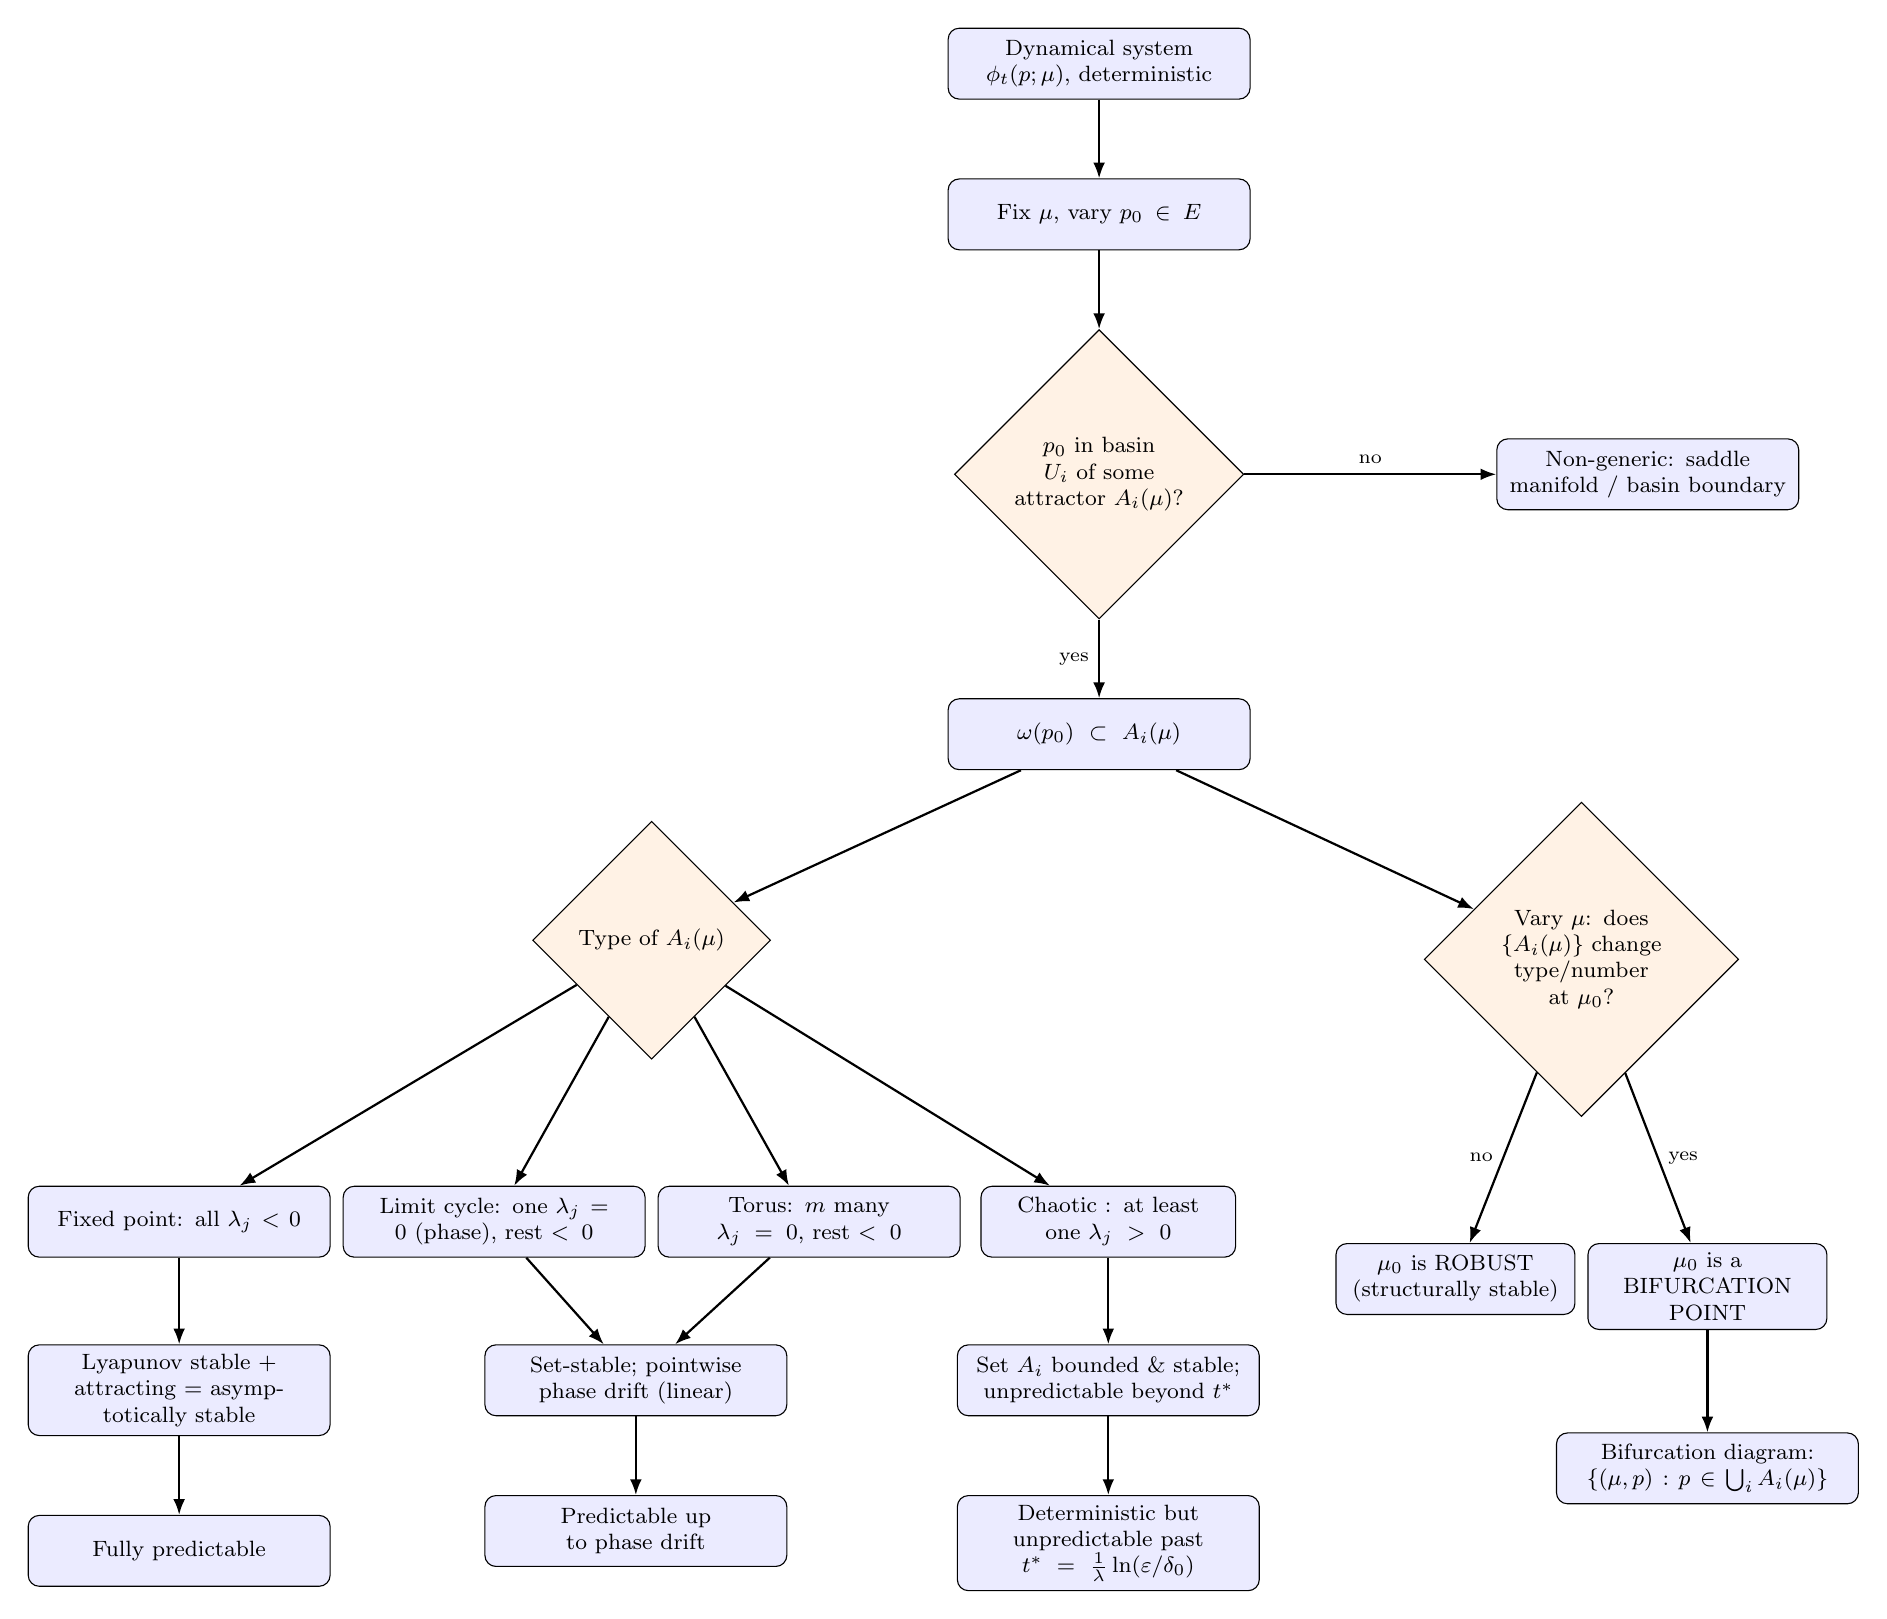
\begin{tikzpicture}[
  node distance=1.0cm and 0.6cm,
  process/.style={rectangle, rounded corners, draw, fill=blue!8, text width=3.6cm, align=center, minimum height=0.9cm, font=\footnotesize},
  decision/.style={diamond, draw, fill=orange!10, text width=2.6cm, align=center, inner sep=1pt, font=\footnotesize},
  arrowstyle/.style={-{Latex[length=2mm]}, thick}
]


\node[process] (A) {Dynamical system $\phi_t(p;\mu)$, deterministic};
\node[process, below=of A] (B) {Fix $\mu$, vary $p_0 \in E$};
\node[decision, below=of B] (C) {$p_0$ in basin $U_i$ of some attractor $A_i(\mu)$?};

\node[process, right=3.2cm of C] (E) {Non-generic: saddle manifold / basin boundary};
\node[process, below=of C] (D) {$\omega(p_0) \subset A_i(\mu)$};

\node[decision, below left=1.4cm and 3.0cm of D] (F) {Type of $A_i(\mu)$};
\node[decision, below right=1.4cm and 3.2cm of D] (I) {Vary $\mu$: does $\{A_i(\mu)\}$ change type/number at $\mu_0$?};


\node[process, below=1.6cm of F, xshift=-6cm] (F1) {Fixed point: all $\lambda_j<0$};
\node[process, below=1.6cm of F, xshift=-2.0cm] (F2) {Limit cycle: one $\lambda_j = 0$ (phase), rest $<0$};
\node[process, below=1.6cm of F, xshift= 2cm]  (F3) {Torus: $m$ many  $\lambda_j =0$, rest $<0$};
\node[process, below=1.6cm of F, xshift=5.8cm, text width=3.0cm]  (F4) {Chaotic : at least one $\lambda_j > 0$};

\node[process, below=1.1cm of F1] (G1) {Lyapunov stable + attracting = asymptotically stable};
\node[process, below=1.1cm of F2, xshift=1.8cm] (G2) {Set-stable; pointwise phase drift (linear)};
\node[process, below=1.1cm of F4] (G3) {Set $A_i$ bounded \& stable; unpredictable beyond $t^*$};

\node[process, below=1.0cm of G1] (H)  {Fully predictable};
\node[process, below=1.0cm of G2] (H2) {Predictable up to phase drift};
\node[process, below=1.0cm of G3] (H3) {Deterministic but unpredictable past $t^* = \tfrac{1}{\lambda}\ln(\varepsilon/\delta_0)$};


\node[process, below=1.6cm of I, xshift=-1.6cm, text width=2.8cm] (J) {$\mu_0$ is ROBUST (structurally stable)};
\node[process, below=1.6cm of I, xshift=1.6cm, text width=2.8cm]  (K) {$\mu_0$ is a \\ BIFURCATION POINT};
\node[process, below=1.3cm of K] (L) {Bifurcation diagram: $\{(\mu,p): p \in \bigcup_i A_i(\mu)\}$};


\draw[arrowstyle] (A) -- (B);
\draw[arrowstyle] (B) -- (C);
\draw[arrowstyle] (C) -- node[left,font=\scriptsize]{yes} (D);
\draw[arrowstyle] (C) -- node[above,font=\scriptsize]{no} (E);

\draw[arrowstyle] (D) -- (F);
\draw[arrowstyle] (D) -- (I);

\draw[arrowstyle] (F) -- (F1);
\draw[arrowstyle] (F) -- (F2);
\draw[arrowstyle] (F) -- (F3);
\draw[arrowstyle] (F) -- (F4);

\draw[arrowstyle] (F1) -- (G1);
\draw[arrowstyle] (F2) -- (G2);
\draw[arrowstyle] (F3) -- (G2);
\draw[arrowstyle] (F4) -- (G3);

\draw[arrowstyle] (G1) -- (H);
\draw[arrowstyle] (G2) -- (H2);
\draw[arrowstyle] (G3) -- (H3);

\draw[arrowstyle] (I) -- node[left,font=\scriptsize]{no} (J);
\draw[arrowstyle] (I) -- node[right,font=\scriptsize]{yes} (K);
\draw[arrowstyle] (K) -- (L);

\end{tikzpicture}
\end{document}